\documentclass[11pt]{article}
\usepackage[utf8]{inputenc}
\usepackage[T1]{fontenc}
\usepackage[margin=1in]{geometry}
\usepackage{amsmath,amssymb}
\usepackage{graphicx}
\usepackage{booktabs}
\usepackage{float}
\usepackage{caption}
\usepackage[hidelinks]{hyperref}

\graphicspath{{figs/}{./}}
\setlength{\parskip}{0.5em}
\setlength{\parindent}{0pt}

\title{Convergence comparison of convex-roof optimisers:\\ GCG (Method I) versus Stiefel (Method II)}
\author{}
\date{\today}
\begin{document}
\maketitle
\section{Setup}
This report compares algorithms for evaluating the genuine multipartite entanglement (GME) of a reduced density matrix $\rho$ via the convex roof. Each algorithm minimises the same objective over pure-state decompositions $\{p_i,|\psi_i\rangle\}$ parameterised by an isometry $U$,
\begin{equation}h(U)=\sum_i p_i\, C_{\mathrm{GME}}\big(|\psi_i\rangle\big),\qquad C_{\mathrm{GME}}(\rho)=\min_{U} h(U).\end{equation}
Results are aggregated from 5 cached files; nothing is recomputed. The quantity of interest is how the cost $h(U)$ decreases with iteration, and whether the methods reach the same minimum.
\begin{table}[H]\centering
\caption{System and optimiser configuration.}
\begin{tabular}{ll}
\toprule
Quantity & Value \\
\midrule
Lattice sites $L$ & 6 \\
Electrons $N_e$ & 6 \\
Interaction $U$ & 4 \\
Hopping $t$ & 1 \\
Mode & uniform \\
Spin-orbitals $n_{\mathrm{so}}$ & 12 \\
Cluster sizes $n$ & 3, 4, 5 \\
Stiefel optimisers compared & L-BFGS-B, Powell, SLSQP, TNC \\
GCG present & yes \\
Restarts per method & 10 \\
Max iterations & varies \\
Ground-state energy $E_0$ & -3.66870618 \\
First-excited energy $E_1$ & -2.89838147 \\
\bottomrule
\end{tabular}
\end{table}
\begin{table}[H]\centering
\caption{Properties of the reduced density matrices used as input.}
\begin{tabular}{cccc c}
\toprule
$n$ & Sites & Purity $\mathrm{Tr}\,\rho^2$ & Entropy $S$ & Num. rank \\
\midrule
3 & (0,1,2) & 0.359322 & 1.257608 & 8 \\
4 & (0,1,2,3) & 0.399589 & 1.309036 & 11 \\
5 & (0,1,2,3,4) & 0.405812 & 1.084780 & 10 \\
\bottomrule
\end{tabular}
\end{table}
\section{Cost versus iteration}
All series minimise the same convex-roof cost $h(U)=\sum_i p_i\,C_{\mathrm{GME}}(|\psi_i\rangle)$. Method\,I is the GCG scheme; Method\,II is the Stiefel-manifold optimiser, here run with sub-optimisers L-BFGS-B, Powell, SLSQP, TNC. The largest spread of final costs across methods and sizes is $3.33\times 10^{-1}$. Recorded iteration counts (history length minus one) span: GCG 300--300; Stiefel L-BFGS-B 6--11; Stiefel Powell 6--9; Stiefel SLSQP 679--889; Stiefel TNC 70--281.
\textbf{Note on the iteration axis.} The horizontal axis counts recorded optimiser steps (callback points). This is a method- and optimiser-specific unit of work: one GCG (Method\,I) step embeds an internal line search, whereas one Stiefel (Method\,II) step is a single iteration of the chosen sub-optimiser (L-BFGS-B, TNC, Powell, \dots), each with its own internal function/gradient evaluations. Iteration \emph{counts} are therefore not directly comparable across methods or across sub-optimisers; the curves below show per-method convergence behaviour, while \emph{efficiency} is compared via final cost and wall-clock time (Section~\ref{sec:summary}). The plotted history is the best restart at the converged cardinality $k$ for each method.
\begin{figure}[H]\centering
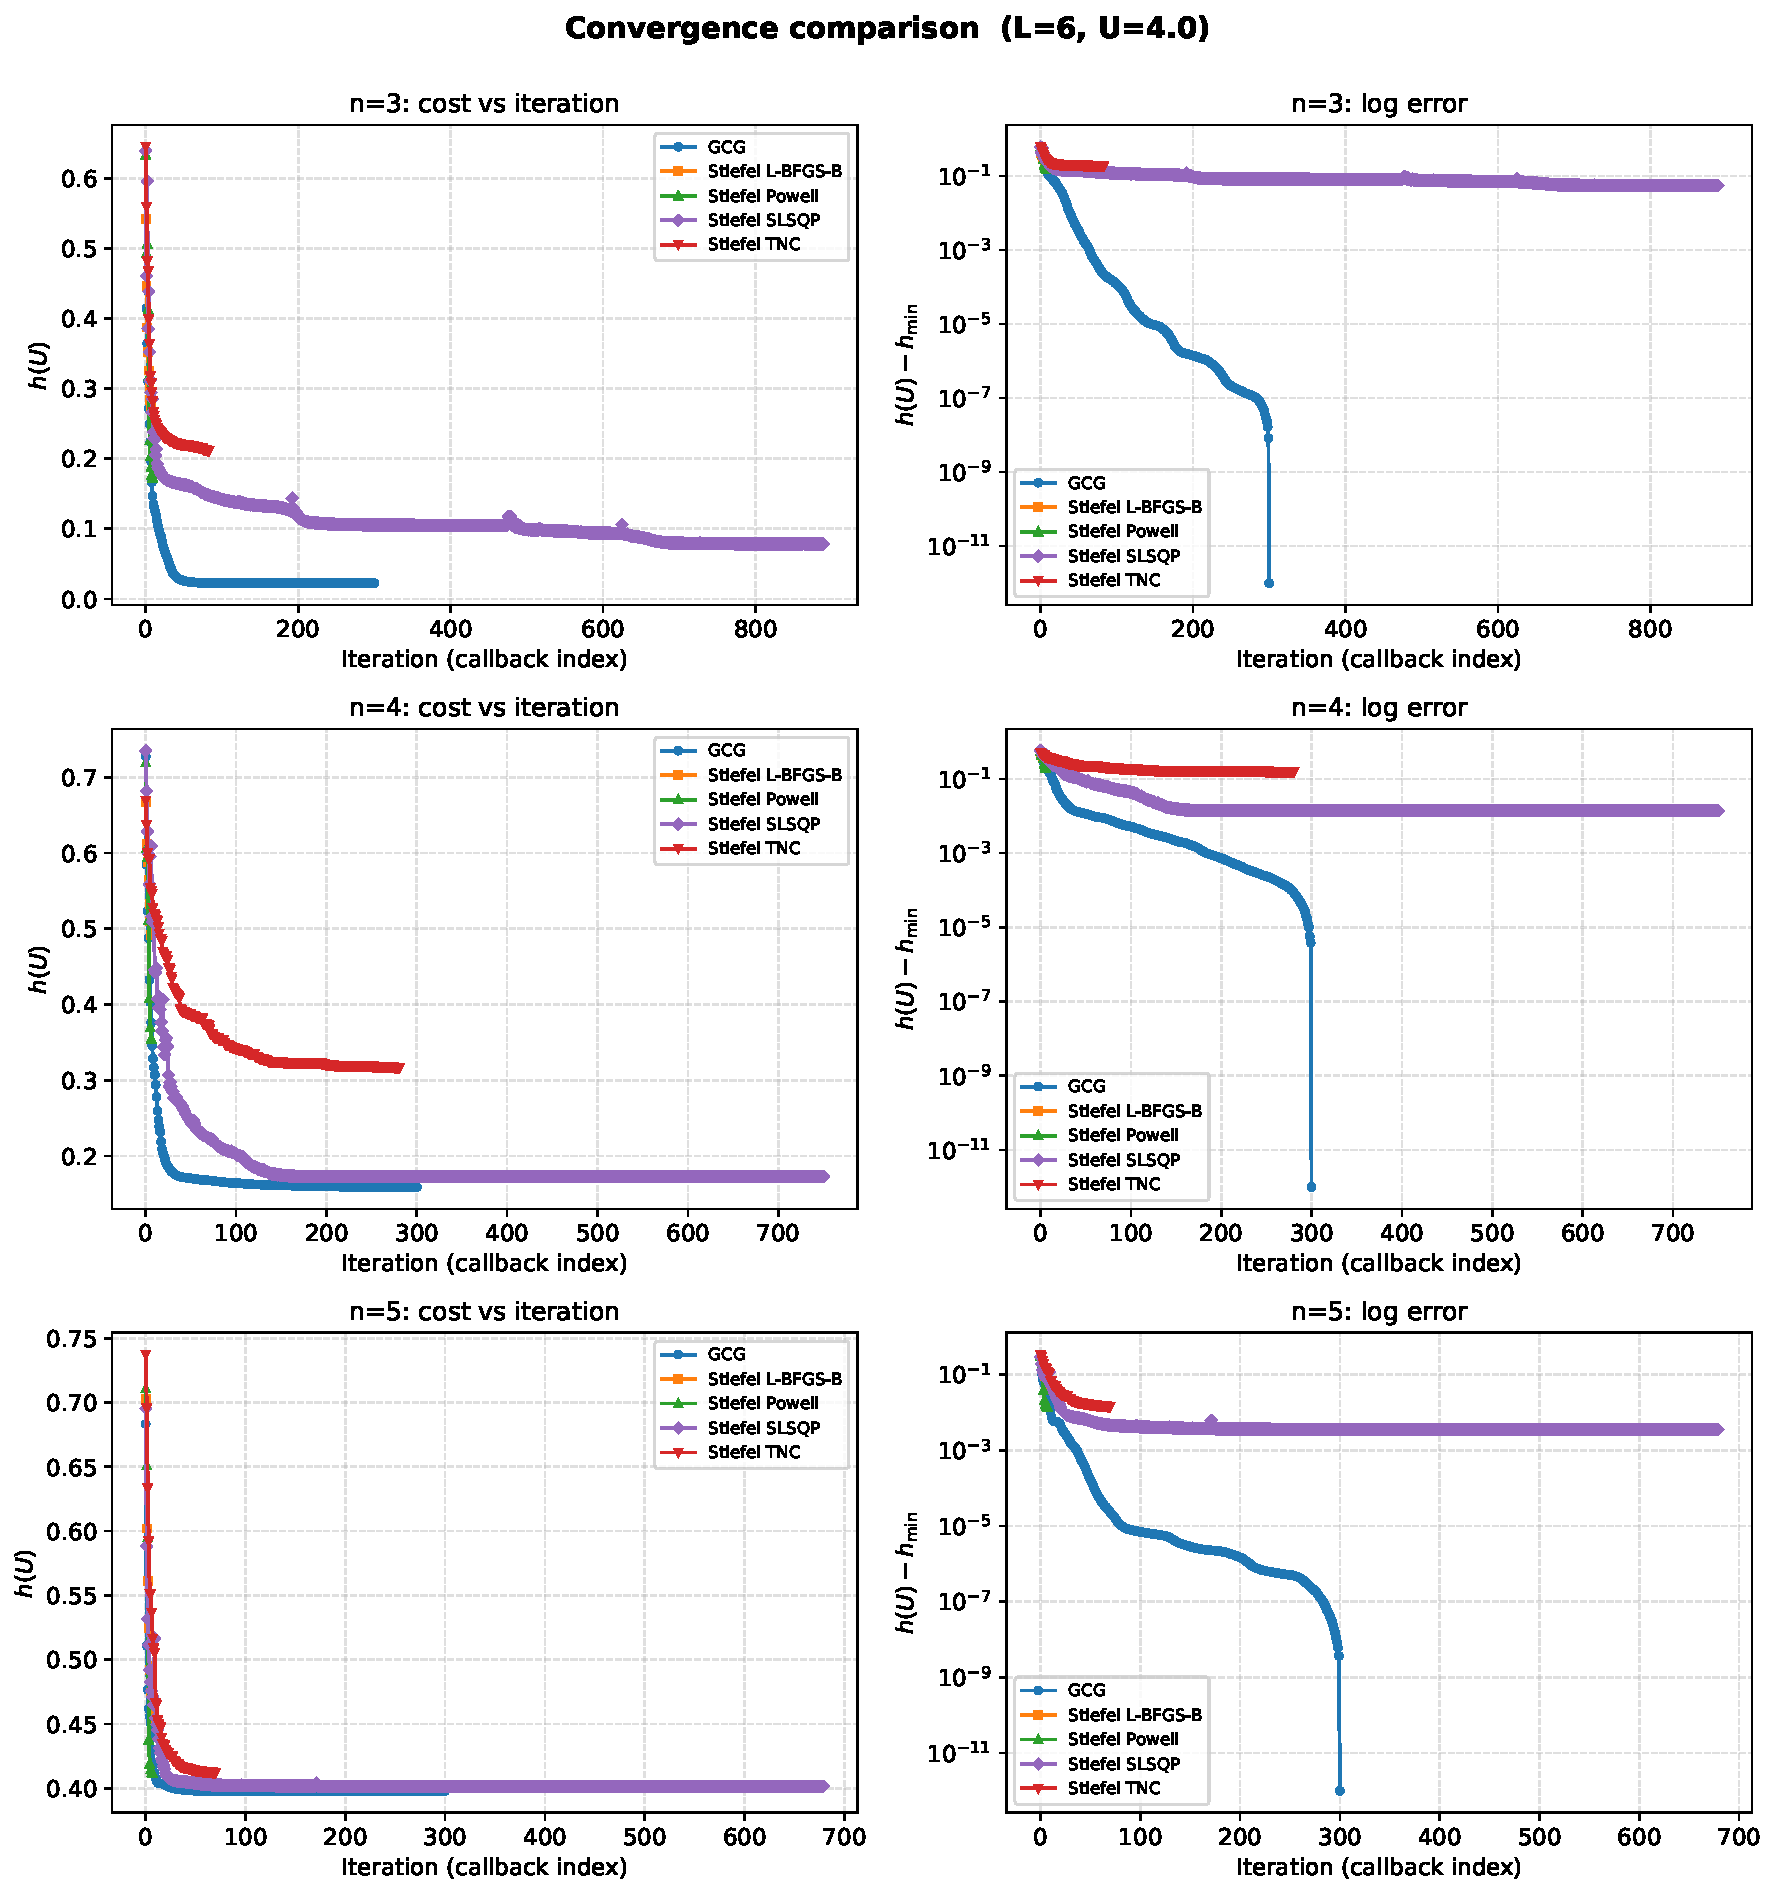
\includegraphics[width=\linewidth]{convergence_combined.pdf}
\caption{Cost $h(U)$ versus iteration (left) and log error $h(U)-h_{\min}$ (right), per cluster size $n$. All available methods are overlaid.}
\label{fig:combined}
\end{figure}
\begin{figure}[H]\centering
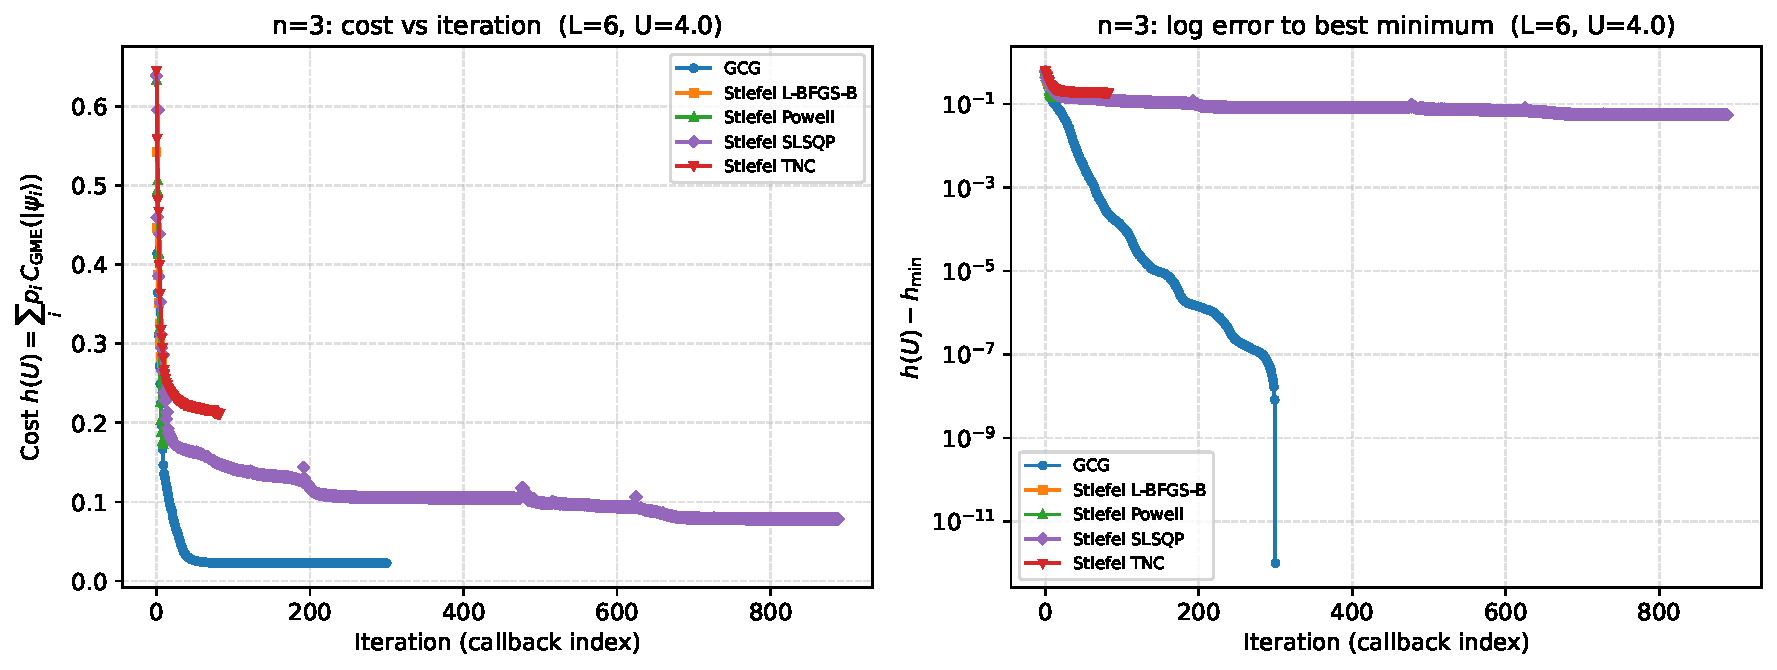
\includegraphics[width=\linewidth]{convergence_n3.pdf}
\caption{$n=3$: cost versus iteration (left) and log error to the best minimum (right).}
\label{fig:n3}
\end{figure}
\begin{figure}[H]\centering
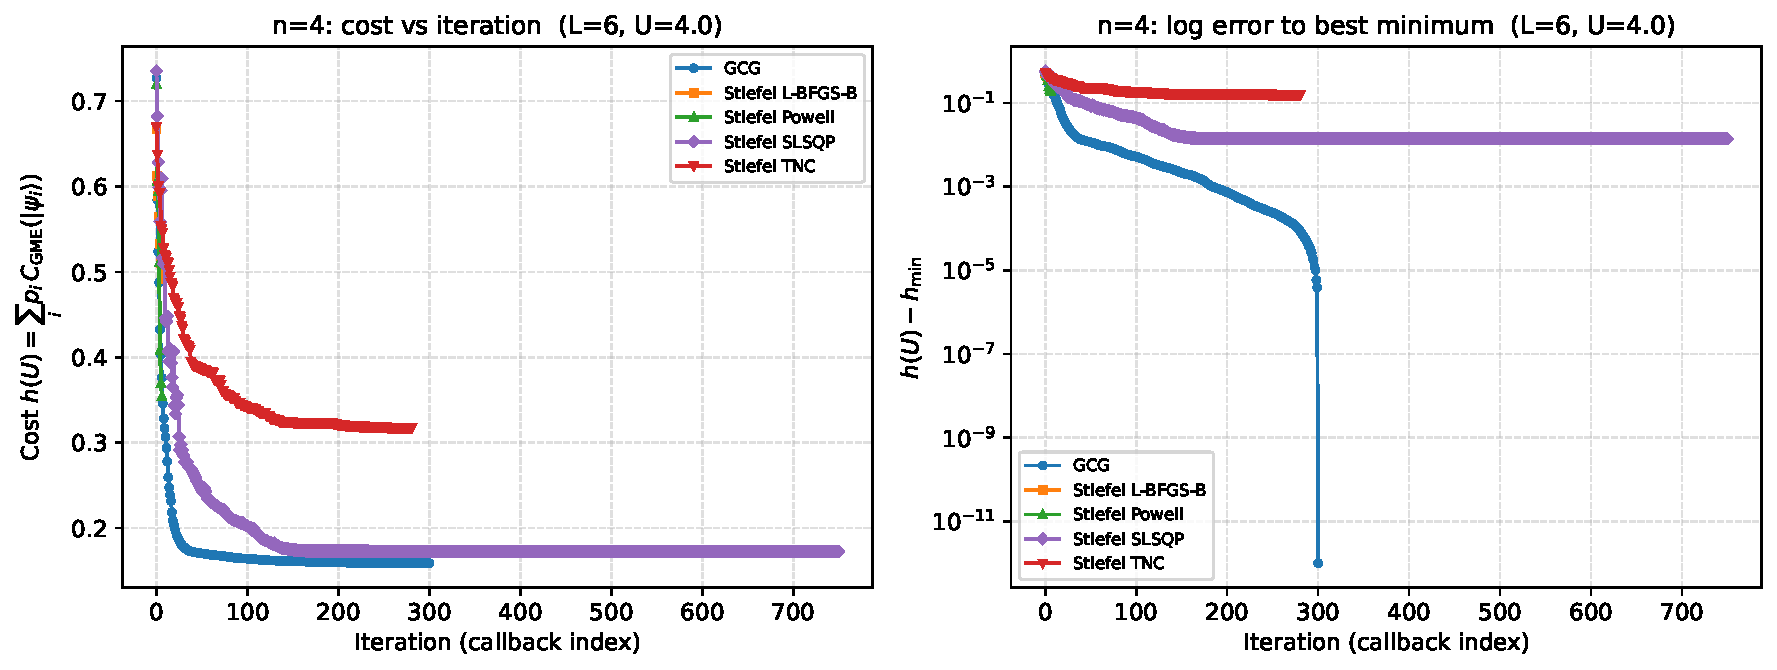
\includegraphics[width=\linewidth]{convergence_n4.pdf}
\caption{$n=4$: cost versus iteration (left) and log error to the best minimum (right).}
\label{fig:n4}
\end{figure}
\begin{figure}[H]\centering
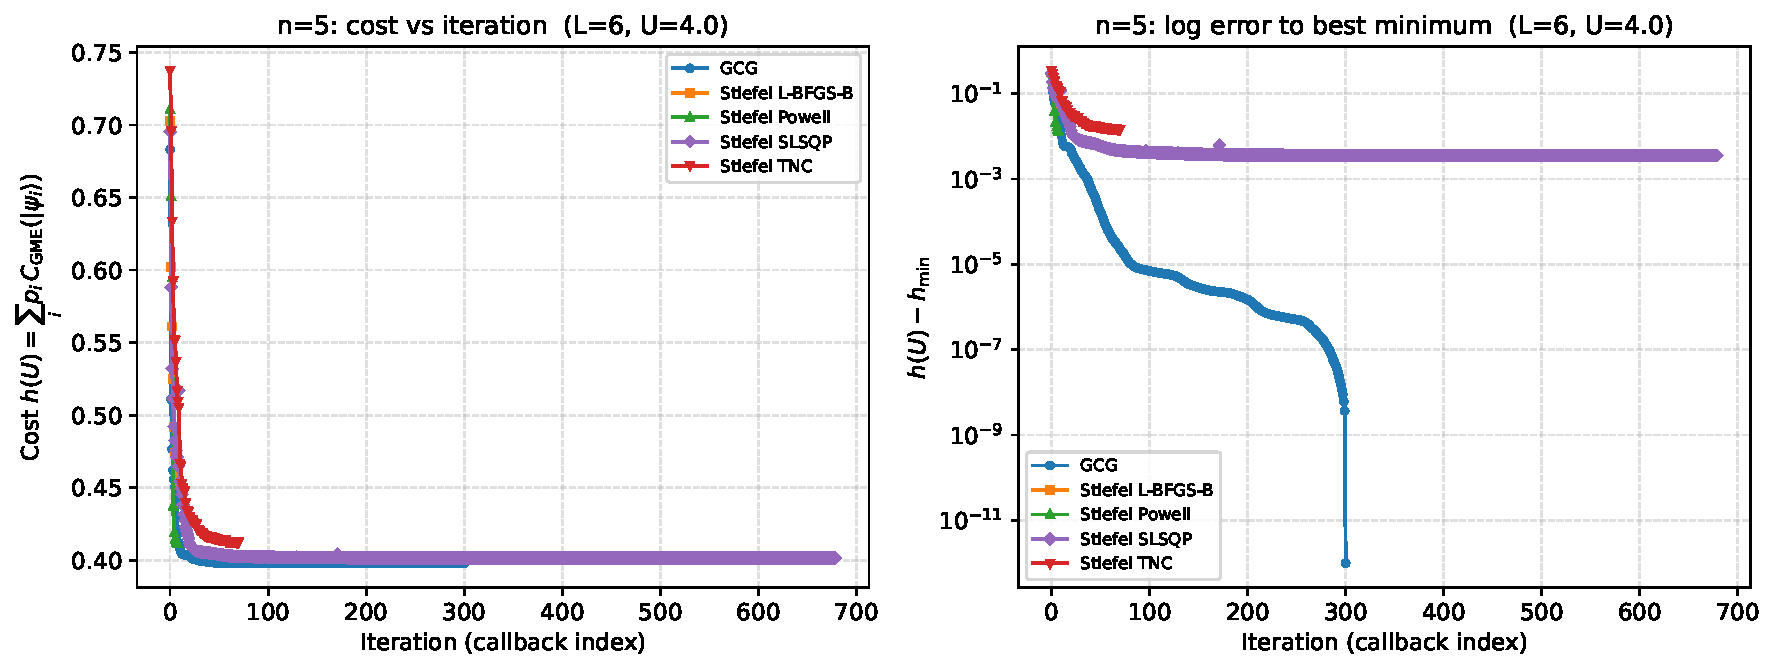
\includegraphics[width=\linewidth]{convergence_n5.pdf}
\caption{$n=5$: cost versus iteration (left) and log error to the best minimum (right).}
\label{fig:n5}
\end{figure}
\subsection{Convergence shape on a common axis}
Because the iteration counts differ between methods and sub-optimisers, the same histories are replotted against the fraction of recorded iterations $\in[0,1]$, which makes the convergence \emph{shape} comparable independently of length.
\begin{figure}[H]\centering
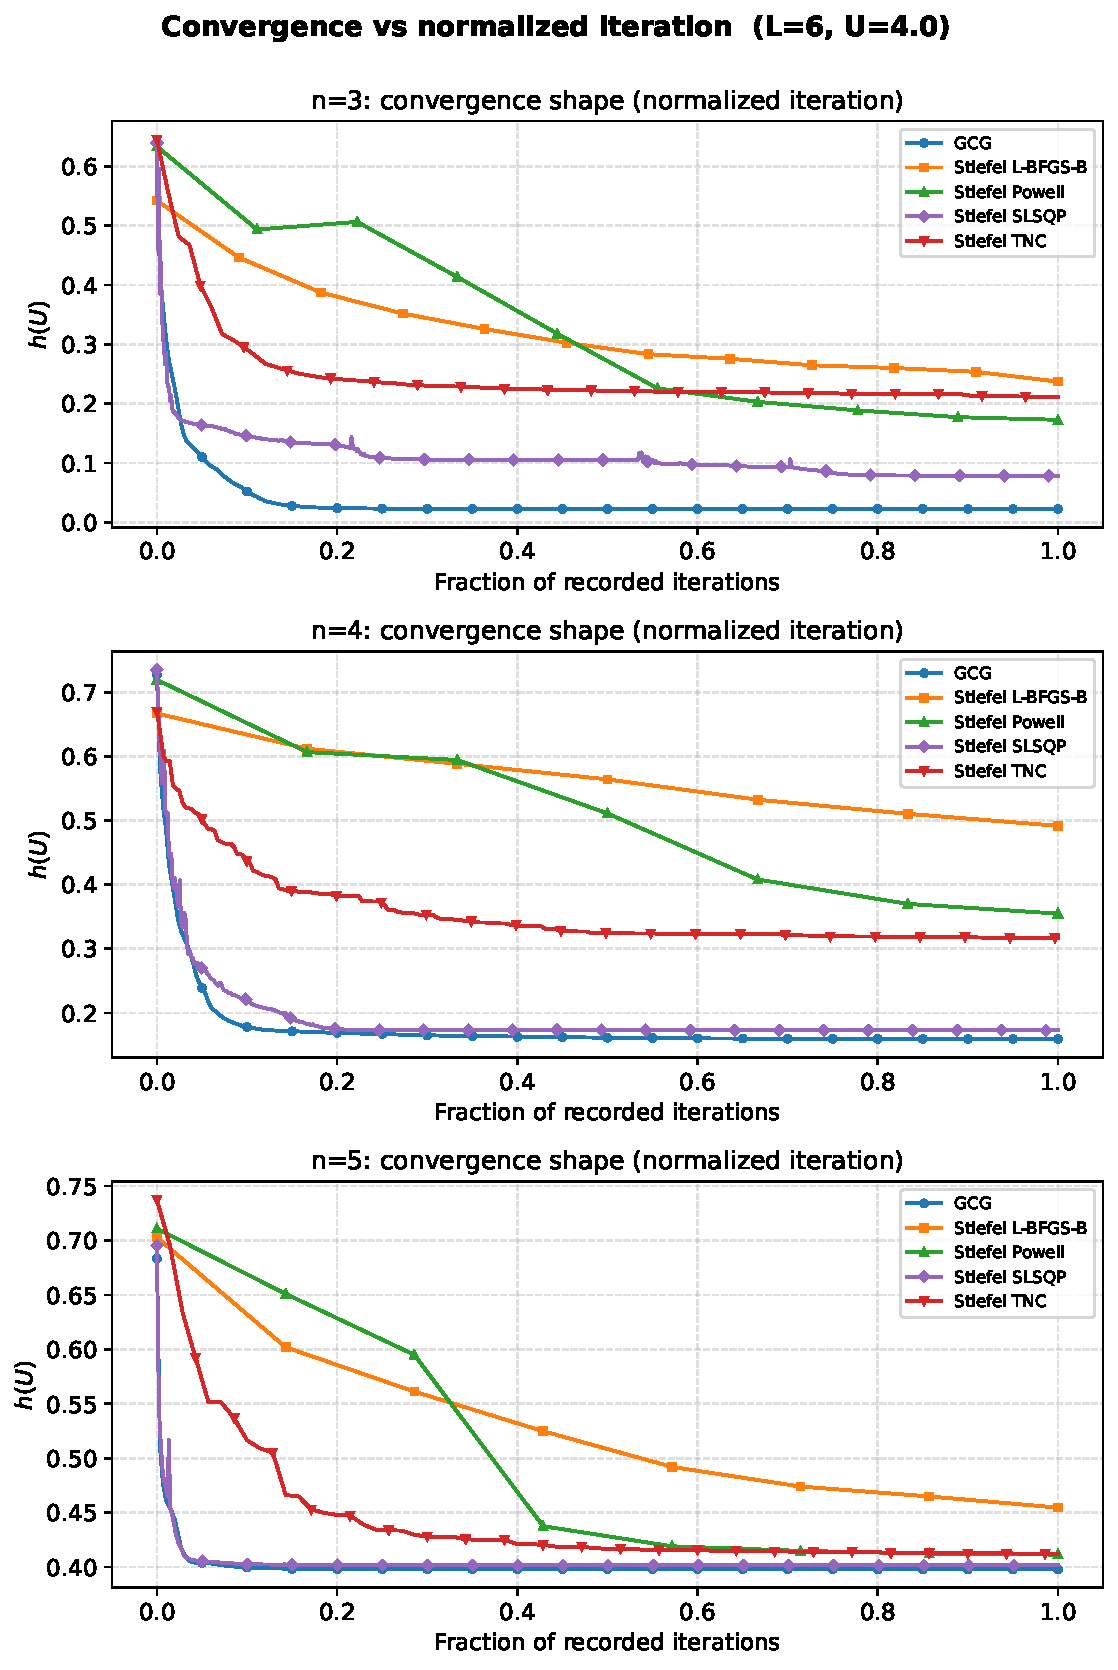
\includegraphics[width=\linewidth]{convergence_normalized.pdf}
\caption{Cost $h(U)$ versus the normalized iteration fraction, per cluster size $n$.}
\label{fig:normalized}
\end{figure}
\section{Summary across cluster size}\label{sec:summary}
Final cost (the estimated $C_{\mathrm{GME}}$), recorded iterations, and wall-clock time per job are summarised below and plotted against $n$.
\begin{table}[H]\centering
\caption{Per-method convergence summary. ``Gap to best'' is the difference between a method's final cost and the lowest final cost at that $n$.}
\begin{tabular}{c l r r r r}
\toprule
$n$ & Method & $h_{\mathrm{final}}$ & Iter. & Time [s] & Gap to best \\
\midrule
3 & GCG (Method\,I) & 0.022500 & 300 & 40.02 & $0$ \\
3 & Stiefel L-BFGS-B (Method\,II) & 0.237089 & 11 & 38.43 & $2.15\times 10^{-1}$ \\
3 & Stiefel Powell (Method\,II) & 0.172739 & 9 & 282.02 & $1.50\times 10^{-1}$ \\
3 & Stiefel SLSQP (Method\,II) & 0.078177 & 889 & 2004.33 & $5.57\times 10^{-2}$ \\
3 & Stiefel TNC (Method\,II) & 0.211808 & 83 & 2252.78 & $1.89\times 10^{-1}$ \\
\midrule
4 & GCG (Method\,I) & 0.159022 & 300 & 764.78 & $0$ \\
4 & Stiefel L-BFGS-B (Method\,II) & 0.491686 & 6 & 85.71 & $3.33\times 10^{-1}$ \\
4 & Stiefel Powell (Method\,II) & 0.354767 & 6 & 680.79 & $1.96\times 10^{-1}$ \\
4 & Stiefel SLSQP (Method\,II) & 0.172897 & 750 & 10218.99 & $1.39\times 10^{-2}$ \\
4 & Stiefel TNC (Method\,II) & 0.316897 & 281 & 10889.27 & $1.58\times 10^{-1}$ \\
\midrule
5 & GCG (Method\,I) & 0.397993 & 300 & 508.52 & $0$ \\
5 & Stiefel L-BFGS-B (Method\,II) & 0.454665 & 7 & 119.61 & $5.67\times 10^{-2}$ \\
5 & Stiefel Powell (Method\,II) & 0.411462 & 7 & 1135.24 & $1.35\times 10^{-2}$ \\
5 & Stiefel SLSQP (Method\,II) & 0.401564 & 679 & 7112.33 & $3.57\times 10^{-3}$ \\
5 & Stiefel TNC (Method\,II) & 0.412330 & 70 & 9243.28 & $1.43\times 10^{-2}$ \\
\bottomrule
\end{tabular}
\end{table}
\begin{figure}[H]\centering
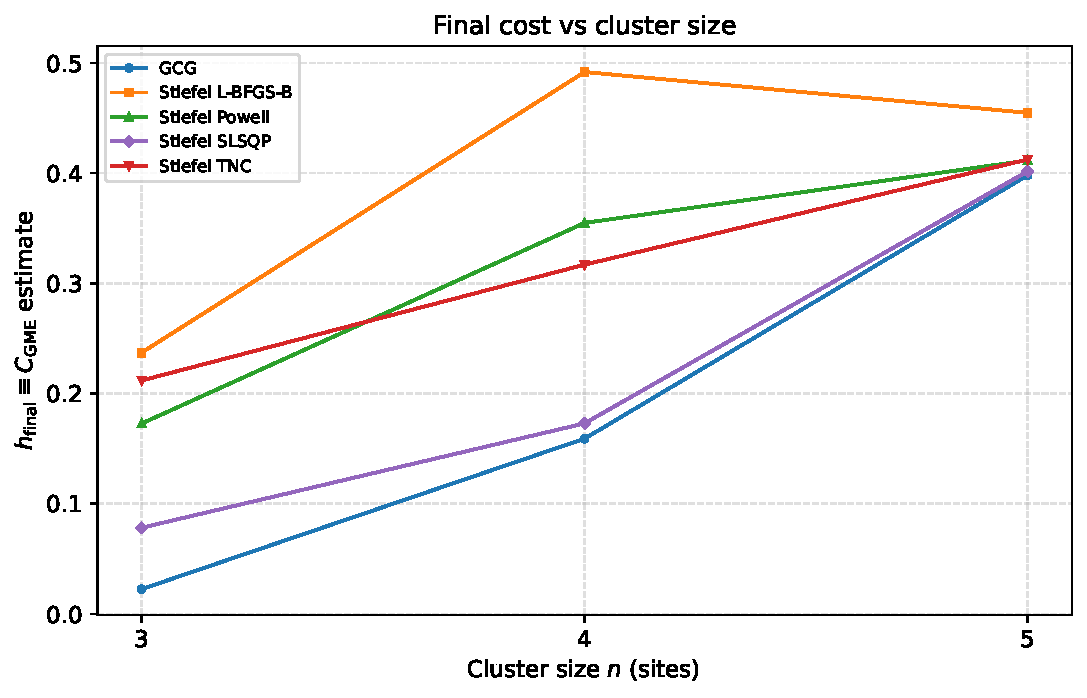
\includegraphics[width=0.78\linewidth]{final_cost_vs_n.pdf}
\caption{Estimated $C_{\mathrm{GME}}$ (final cost) versus cluster size $n$.}
\end{figure}
\begin{figure}[H]\centering
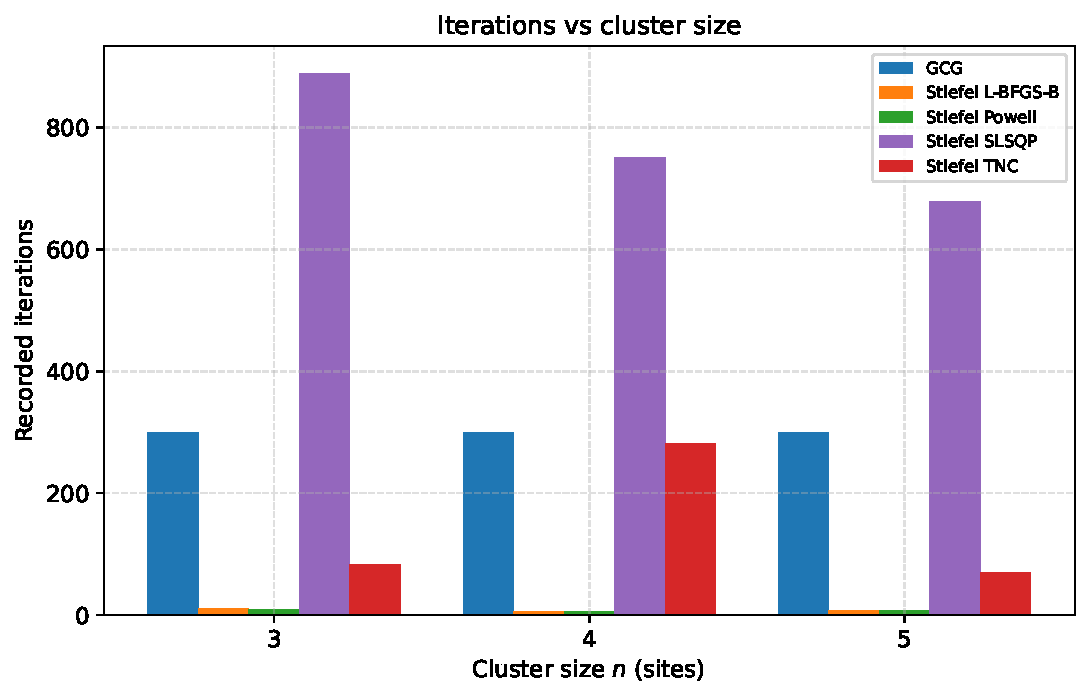
\includegraphics[width=0.78\linewidth]{iterations_vs_n.pdf}
\caption{Recorded iteration count versus cluster size $n$.}
\end{figure}
\begin{figure}[H]\centering
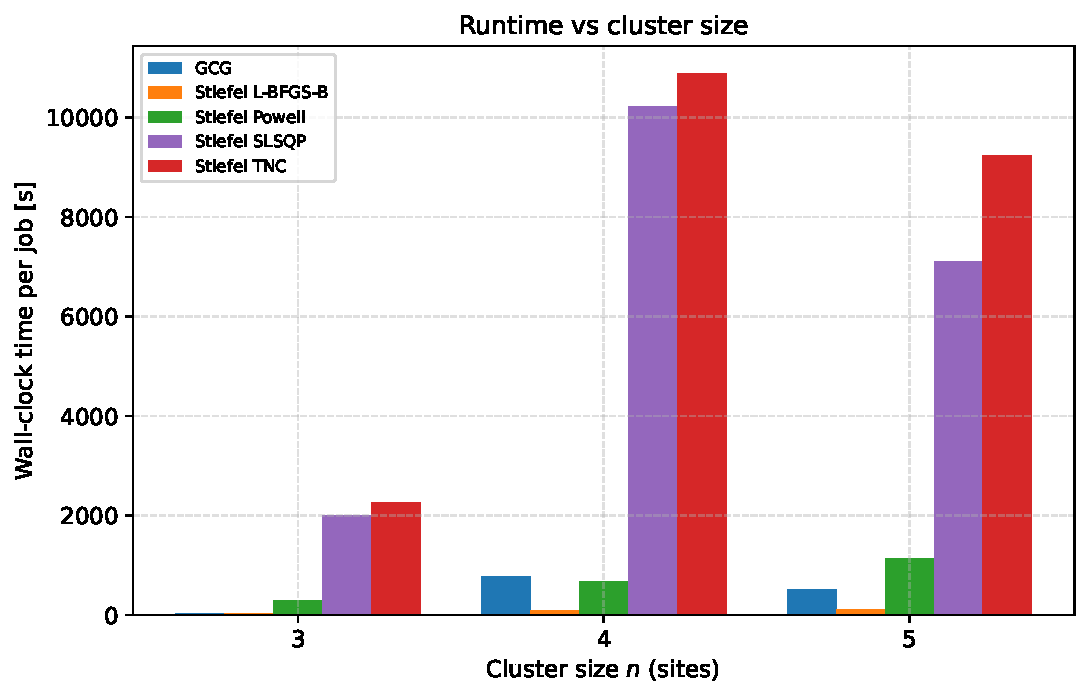
\includegraphics[width=0.78\linewidth]{runtime_vs_n.pdf}
\caption{Wall-clock time per job versus cluster size $n$.}
\end{figure}
\subsection{Cross-method efficiency: cost vs wall-clock time}
Since iteration counts are not a common currency, the fair efficiency comparison is the final cost reached against the wall-clock time spent. Points toward the lower-left (low cost, low time) are preferable; points at the same height indicate methods that reach the same minimum at different cost in time.
\begin{figure}[H]\centering
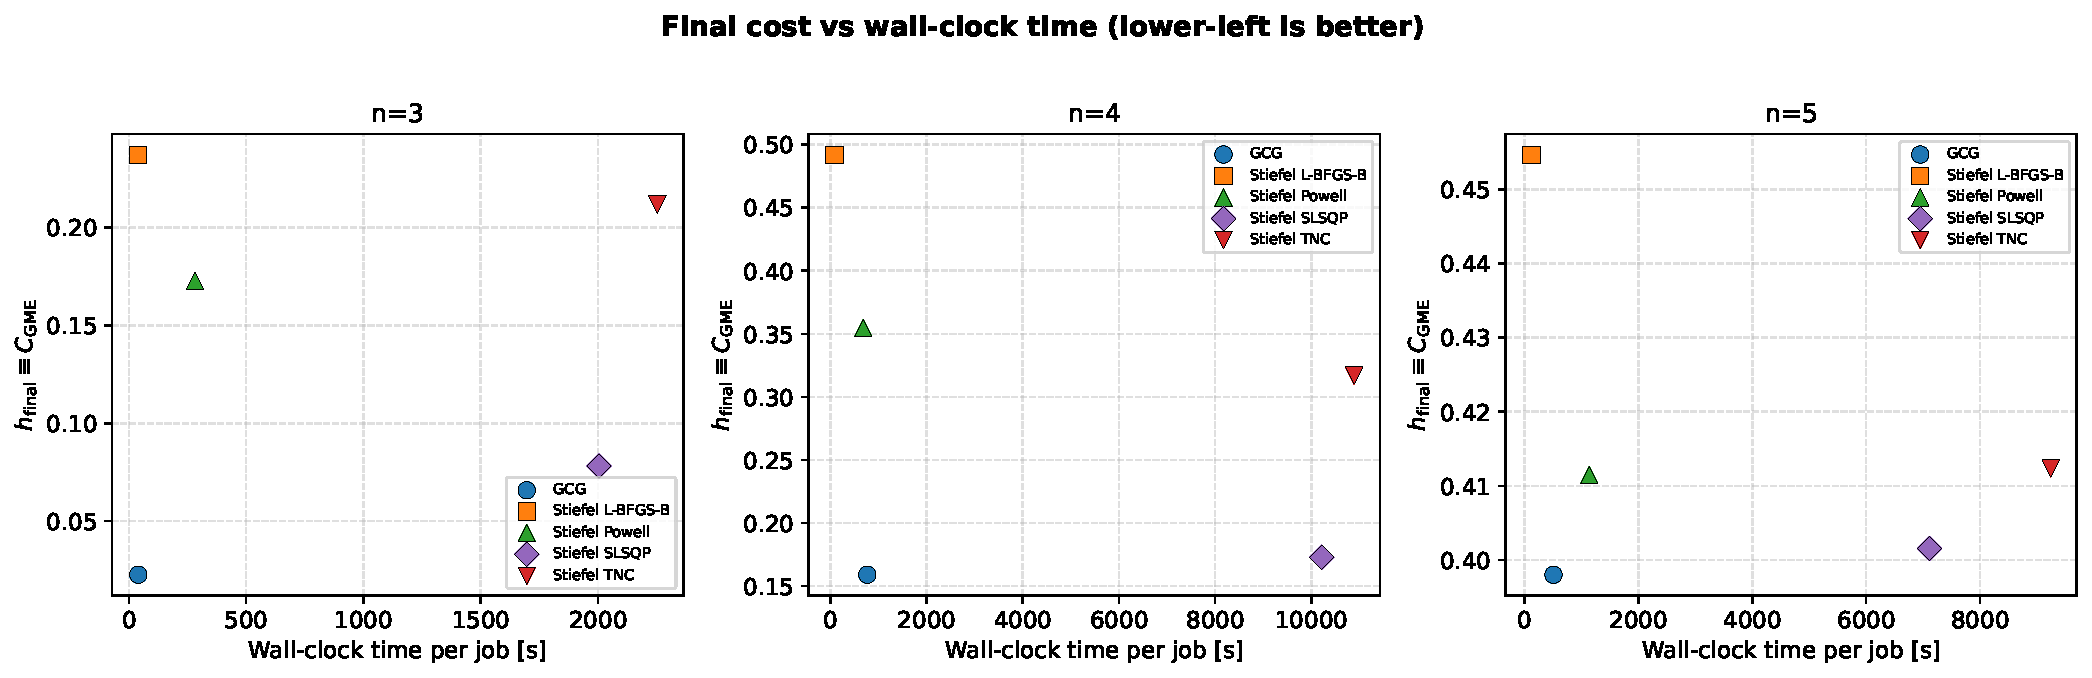
\includegraphics[width=\linewidth]{final_cost_vs_time.pdf}
\caption{Final cost $h_{\mathrm{final}}$ versus wall-clock time per job, faceted by cluster size $n$.}
\label{fig:cost_vs_time}
\end{figure}
\section{Stiefel outer-loop convergence}
Where the Stiefel optimiser records an outer $k$-loop, its convergence is shown below.
\begin{figure}[H]\centering
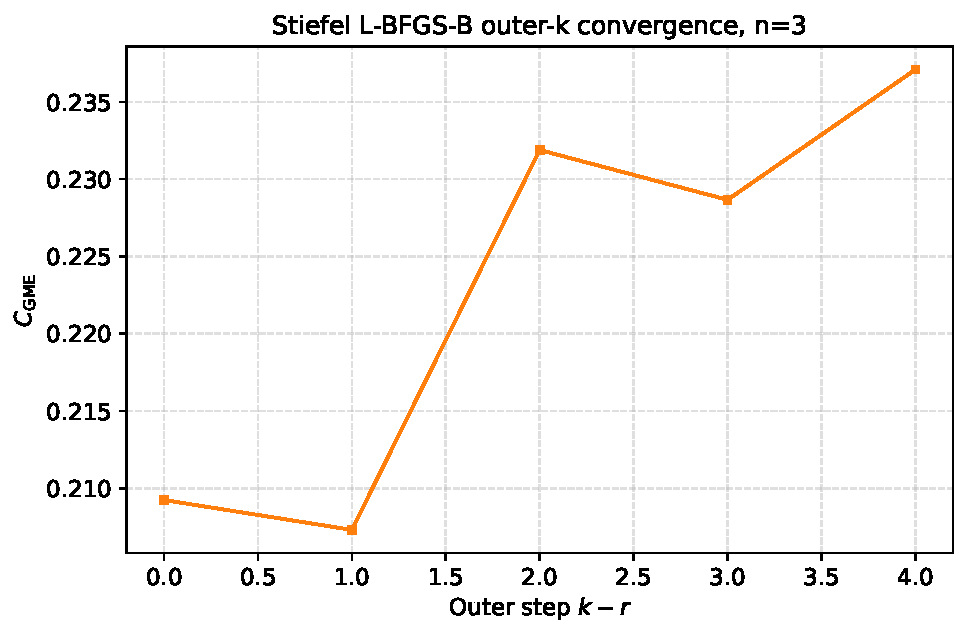
\includegraphics[width=0.58\linewidth]{stiefel_outer_k_L-BFGS-B_n3.pdf}
\caption{Stiefel L-BFGS-B outer-$k$ convergence, $n=3$.}
\end{figure}
\begin{figure}[H]\centering
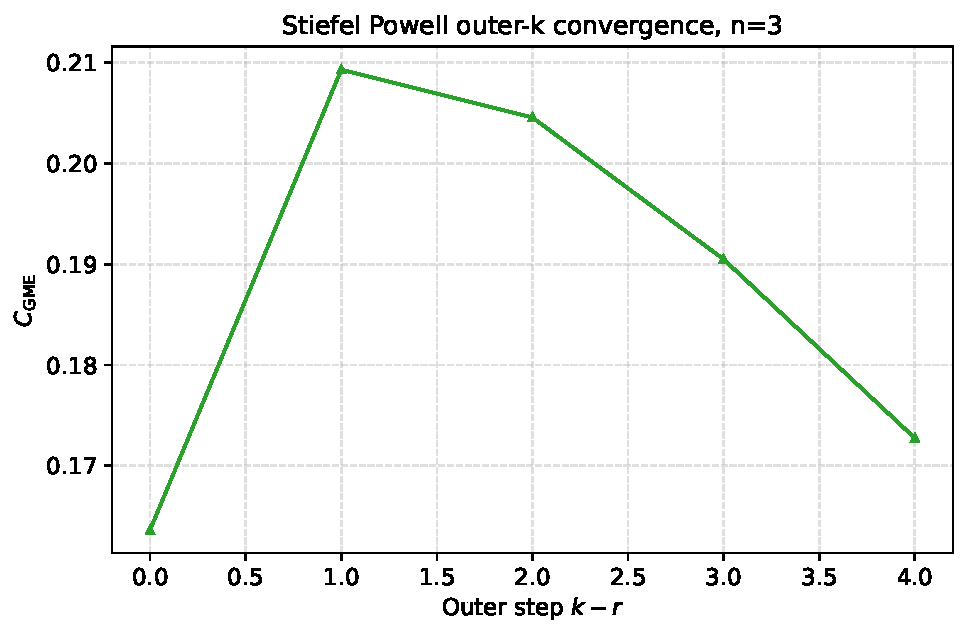
\includegraphics[width=0.58\linewidth]{stiefel_outer_k_Powell_n3.pdf}
\caption{Stiefel Powell outer-$k$ convergence, $n=3$.}
\end{figure}
\begin{figure}[H]\centering
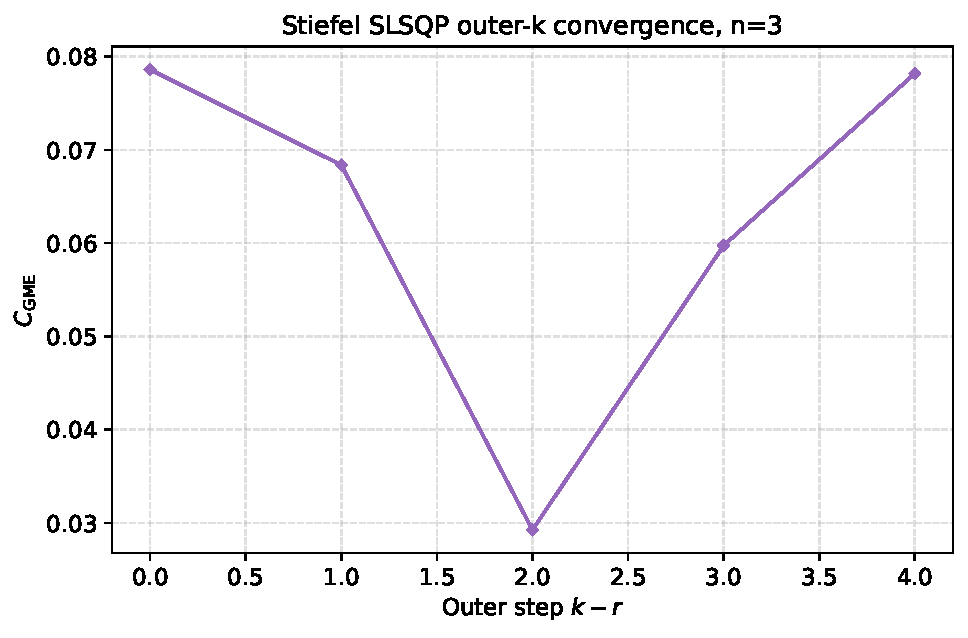
\includegraphics[width=0.58\linewidth]{stiefel_outer_k_SLSQP_n3.pdf}
\caption{Stiefel SLSQP outer-$k$ convergence, $n=3$.}
\end{figure}
\begin{figure}[H]\centering
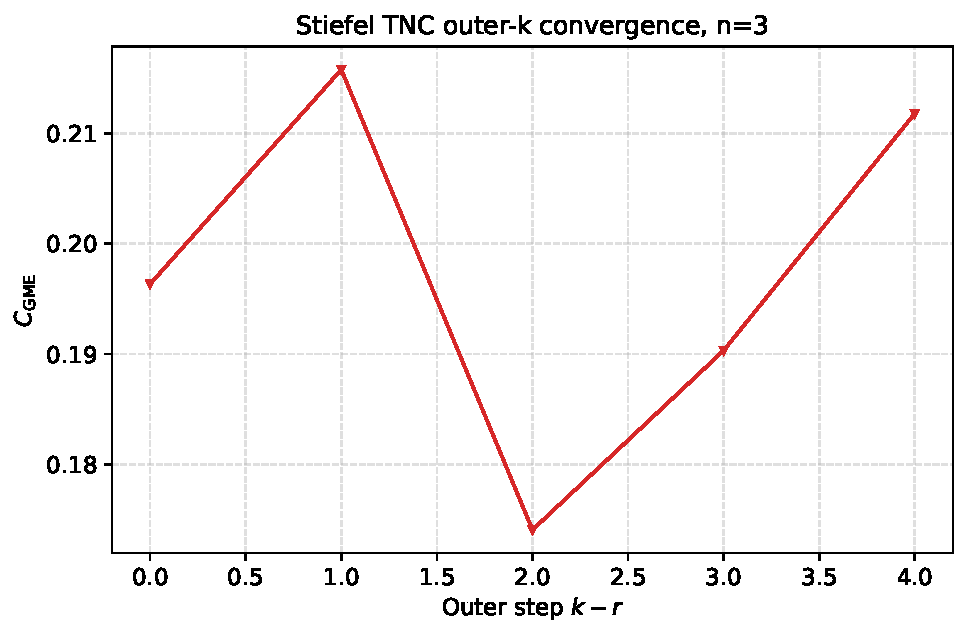
\includegraphics[width=0.58\linewidth]{stiefel_outer_k_TNC_n3.pdf}
\caption{Stiefel TNC outer-$k$ convergence, $n=3$.}
\end{figure}
\begin{figure}[H]\centering
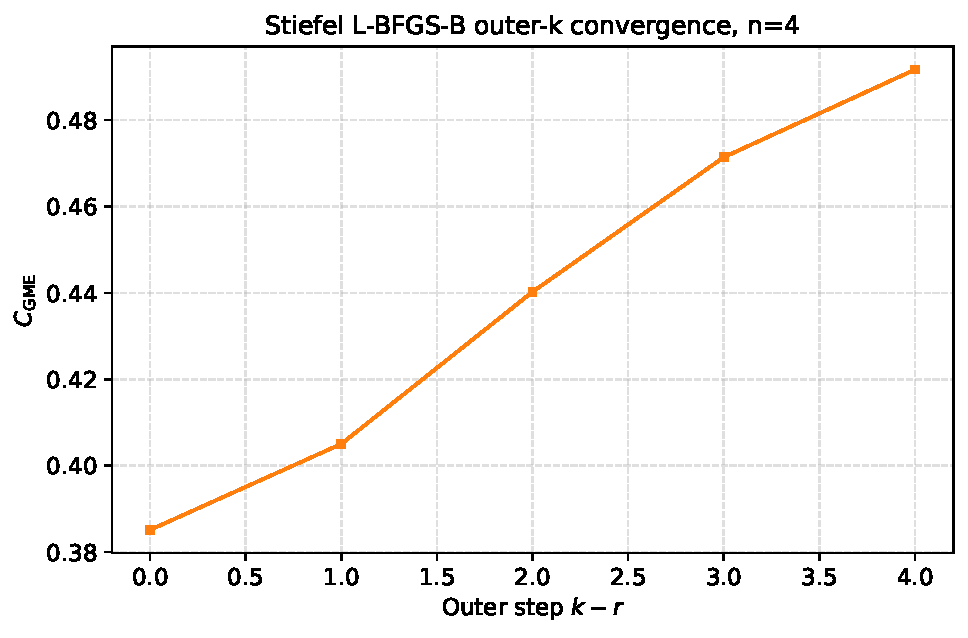
\includegraphics[width=0.58\linewidth]{stiefel_outer_k_L-BFGS-B_n4.pdf}
\caption{Stiefel L-BFGS-B outer-$k$ convergence, $n=4$.}
\end{figure}
\begin{figure}[H]\centering
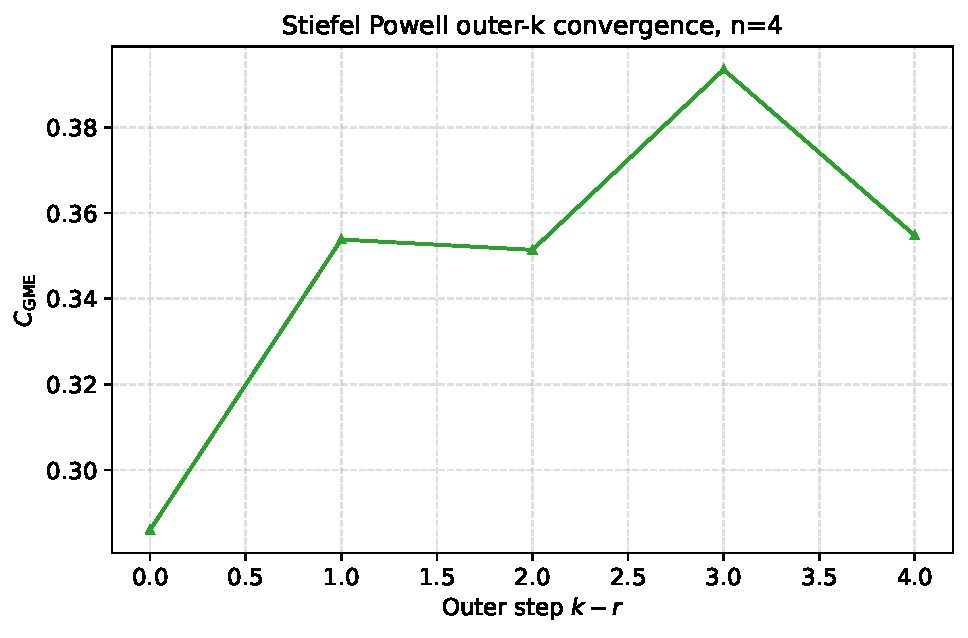
\includegraphics[width=0.58\linewidth]{stiefel_outer_k_Powell_n4.pdf}
\caption{Stiefel Powell outer-$k$ convergence, $n=4$.}
\end{figure}
\begin{figure}[H]\centering
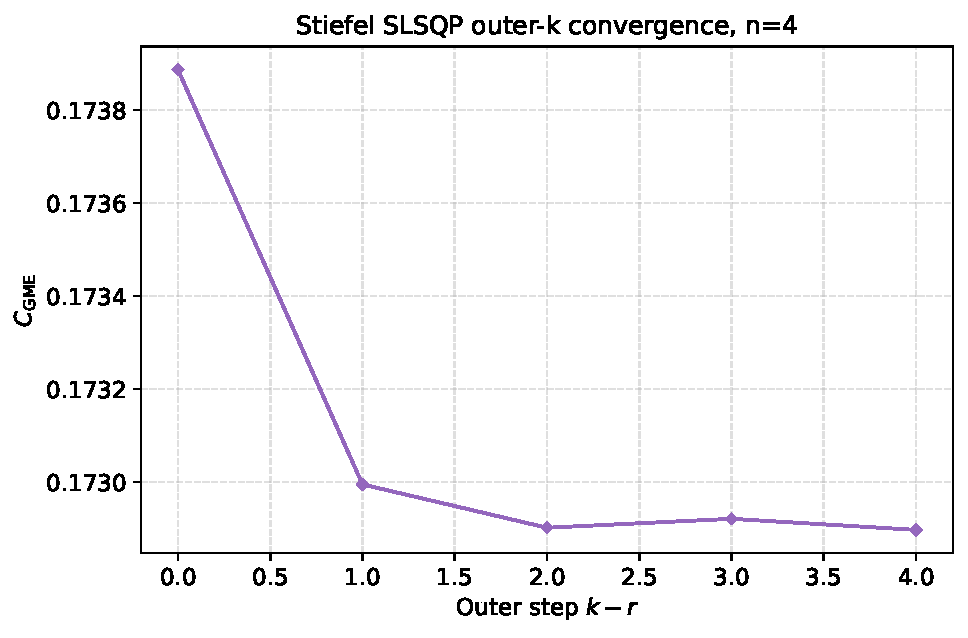
\includegraphics[width=0.58\linewidth]{stiefel_outer_k_SLSQP_n4.pdf}
\caption{Stiefel SLSQP outer-$k$ convergence, $n=4$.}
\end{figure}
\begin{figure}[H]\centering
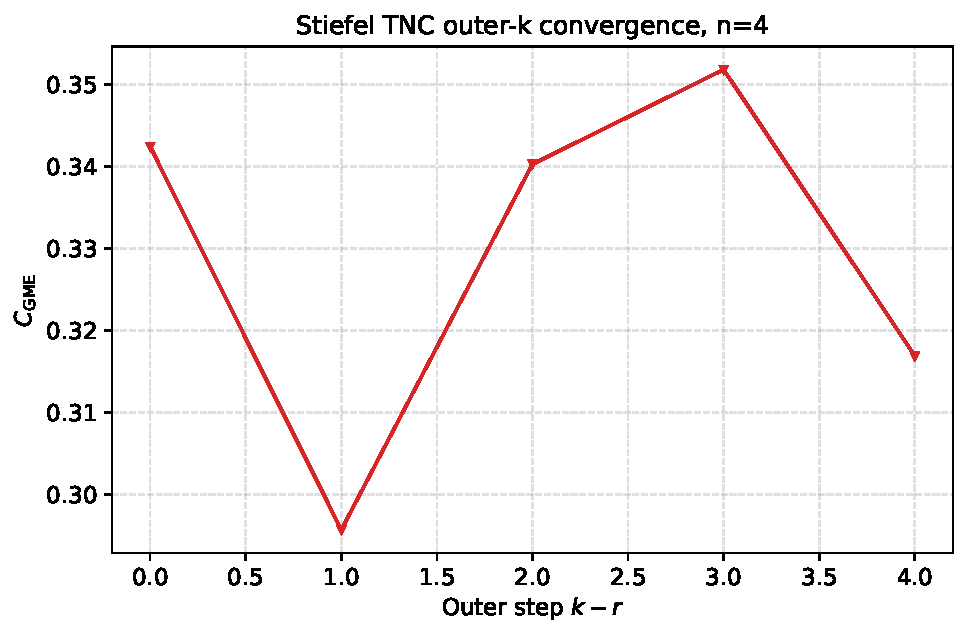
\includegraphics[width=0.58\linewidth]{stiefel_outer_k_TNC_n4.pdf}
\caption{Stiefel TNC outer-$k$ convergence, $n=4$.}
\end{figure}
\begin{figure}[H]\centering
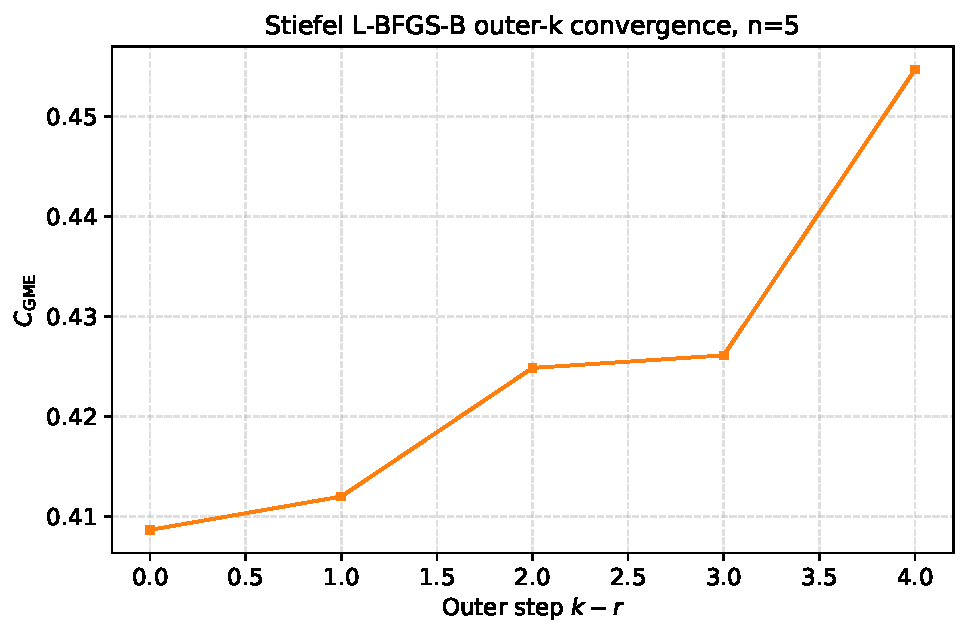
\includegraphics[width=0.58\linewidth]{stiefel_outer_k_L-BFGS-B_n5.pdf}
\caption{Stiefel L-BFGS-B outer-$k$ convergence, $n=5$.}
\end{figure}
\begin{figure}[H]\centering
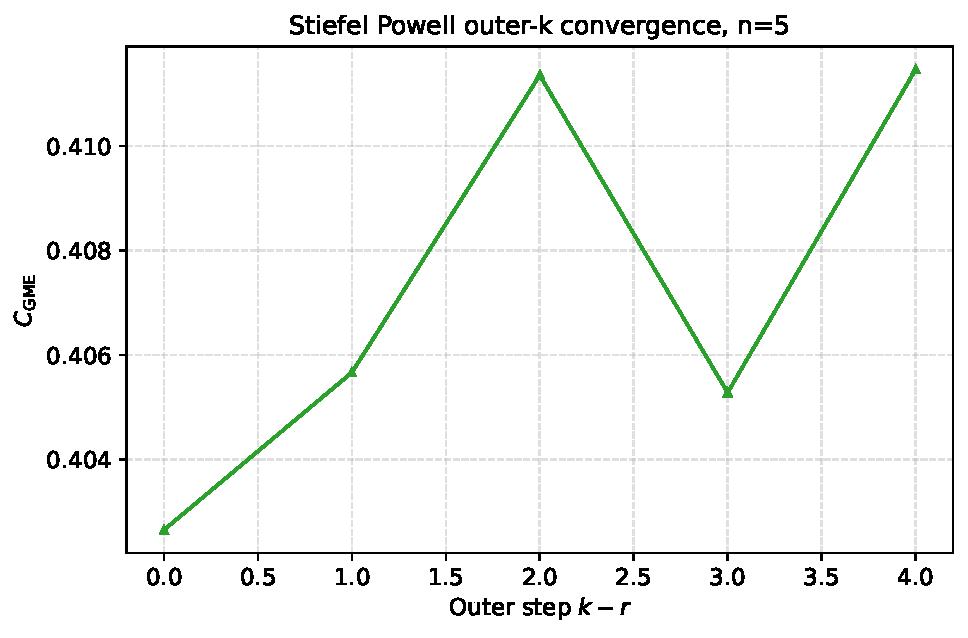
\includegraphics[width=0.58\linewidth]{stiefel_outer_k_Powell_n5.pdf}
\caption{Stiefel Powell outer-$k$ convergence, $n=5$.}
\end{figure}
\begin{figure}[H]\centering
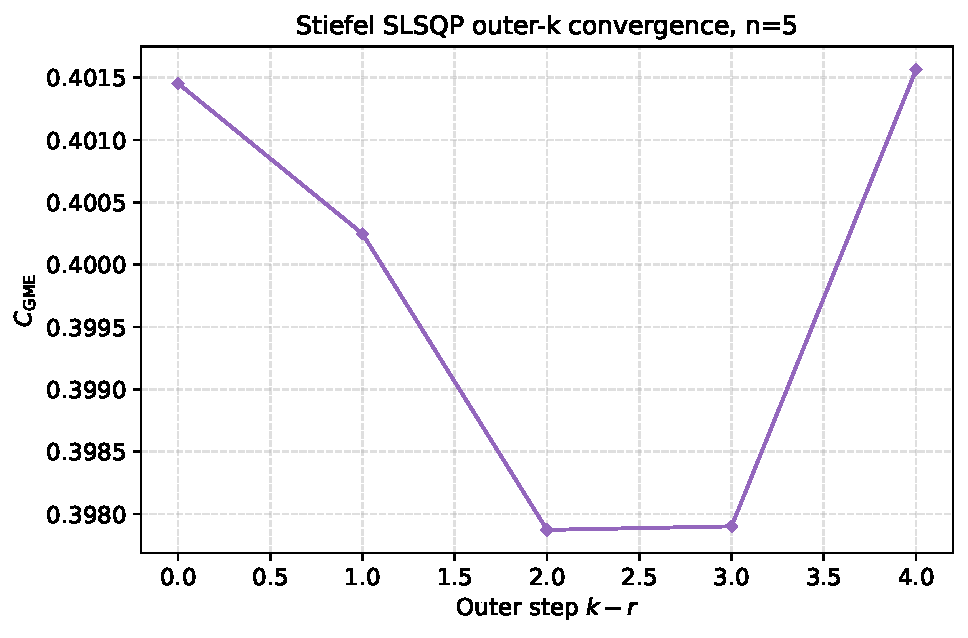
\includegraphics[width=0.58\linewidth]{stiefel_outer_k_SLSQP_n5.pdf}
\caption{Stiefel SLSQP outer-$k$ convergence, $n=5$.}
\end{figure}
\begin{figure}[H]\centering
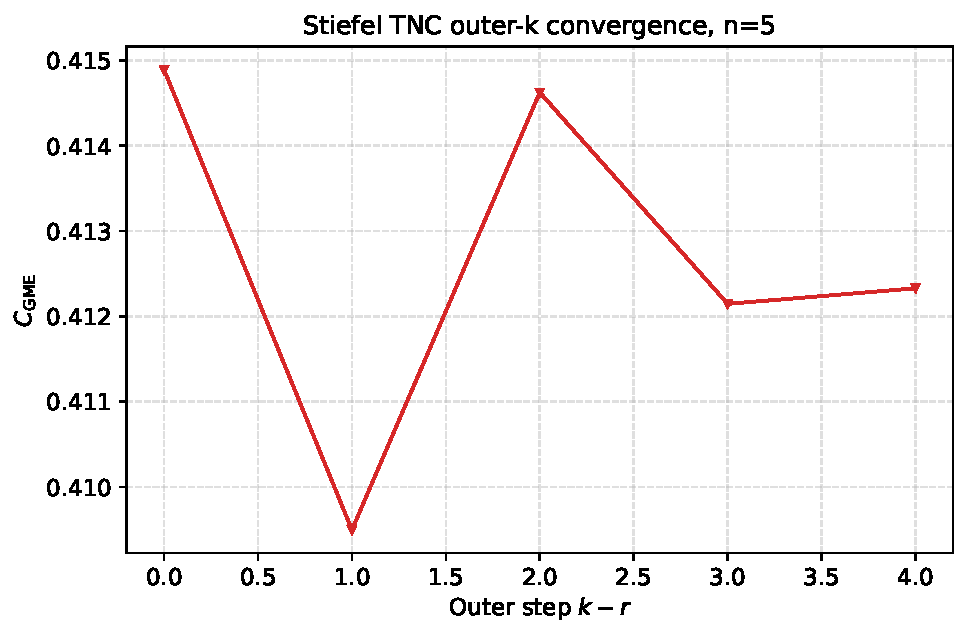
\includegraphics[width=0.58\linewidth]{stiefel_outer_k_TNC_n5.pdf}
\caption{Stiefel TNC outer-$k$ convergence, $n=5$.}
\end{figure}
\section*{Appendix: data provenance}
Each result is tagged by how it entered its cached file (\texttt{computed}, \texttt{job\_cache}, or \texttt{full\_pkl}) and by the file it came from.
\begin{table}[H]\centering
\caption{Provenance of each stored result.}
\begin{tabular}{c l l l}
\toprule
$n$ & Method & Source & File \\
\midrule
3 & GCG (Method\,I) & computed & {\scriptsize\texttt{conv\_v1\_L6\_Ne6\_nso12\_U4\_t1\_mode-uniform\_n3-4-5\_methods-all\_method-II-L-BFGS-B\_restarts10\_iter300\_20260619\_001046.pkl}} \\
3 & Stiefel L-BFGS-B (Method\,II) & computed & {\scriptsize\texttt{conv\_v1\_L6\_Ne6\_nso12\_U4\_t1\_mode-uniform\_n3-4-5\_methods-all\_method-II-L-BFGS-B\_restarts10\_iter300\_20260619\_001046.pkl}} \\
3 & Stiefel Powell (Method\,II) & computed & {\scriptsize\texttt{conv\_v1\_L6\_Ne6\_nso12\_U4\_t1\_mode-uniform\_n3-4-5\_methods-stiefel\_stiefel-Powell\_restarts10\_iter5000\_20260605\_111551.pkl}} \\
3 & Stiefel SLSQP (Method\,II) & computed & {\scriptsize\texttt{conv\_v1\_L6\_Ne6\_nso12\_U4\_t1\_mode-uniform\_n3-4-5\_methods-stiefel\_stiefel-SLSQP\_restarts10\_iter5000\_20260605\_113302.pkl}} \\
3 & Stiefel TNC (Method\,II) & computed & {\scriptsize\texttt{conv\_v1\_L6\_Ne6\_nso12\_U4\_t1\_mode-uniform\_n3-4-5\_methods-stiefel\_stiefel-TNC\_restarts10\_iter5000\_20260605\_114629.pkl}} \\
4 & GCG (Method\,I) & computed & {\scriptsize\texttt{conv\_v1\_L6\_Ne6\_nso12\_U4\_t1\_mode-uniform\_n3-4-5\_methods-all\_method-II-L-BFGS-B\_restarts10\_iter300\_20260619\_001046.pkl}} \\
4 & Stiefel L-BFGS-B (Method\,II) & computed & {\scriptsize\texttt{conv\_v1\_L6\_Ne6\_nso12\_U4\_t1\_mode-uniform\_n3-4-5\_methods-all\_method-II-L-BFGS-B\_restarts10\_iter300\_20260619\_001046.pkl}} \\
4 & Stiefel Powell (Method\,II) & computed & {\scriptsize\texttt{conv\_v1\_L6\_Ne6\_nso12\_U4\_t1\_mode-uniform\_n3-4-5\_methods-stiefel\_stiefel-Powell\_restarts10\_iter5000\_20260605\_111551.pkl}} \\
4 & Stiefel SLSQP (Method\,II) & computed & {\scriptsize\texttt{conv\_v1\_L6\_Ne6\_nso12\_U4\_t1\_mode-uniform\_n3-4-5\_methods-stiefel\_stiefel-SLSQP\_restarts10\_iter5000\_20260605\_113302.pkl}} \\
4 & Stiefel TNC (Method\,II) & computed & {\scriptsize\texttt{conv\_v1\_L6\_Ne6\_nso12\_U4\_t1\_mode-uniform\_n3-4-5\_methods-stiefel\_stiefel-TNC\_restarts10\_iter5000\_20260605\_114629.pkl}} \\
5 & GCG (Method\,I) & computed & {\scriptsize\texttt{conv\_v1\_L6\_Ne6\_nso12\_U4\_t1\_mode-uniform\_n3-4-5\_methods-all\_method-II-L-BFGS-B\_restarts10\_iter300\_20260619\_001046.pkl}} \\
5 & Stiefel L-BFGS-B (Method\,II) & computed & {\scriptsize\texttt{conv\_v1\_L6\_Ne6\_nso12\_U4\_t1\_mode-uniform\_n3-4-5\_methods-all\_method-II-L-BFGS-B\_restarts10\_iter300\_20260619\_001046.pkl}} \\
5 & Stiefel Powell (Method\,II) & computed & {\scriptsize\texttt{conv\_v1\_L6\_Ne6\_nso12\_U4\_t1\_mode-uniform\_n3-4-5\_methods-stiefel\_stiefel-Powell\_restarts10\_iter5000\_20260605\_111551.pkl}} \\
5 & Stiefel SLSQP (Method\,II) & computed & {\scriptsize\texttt{conv\_v1\_L6\_Ne6\_nso12\_U4\_t1\_mode-uniform\_n3-4-5\_methods-stiefel\_stiefel-SLSQP\_restarts10\_iter5000\_20260605\_113302.pkl}} \\
5 & Stiefel TNC (Method\,II) & computed & {\scriptsize\texttt{conv\_v1\_L6\_Ne6\_nso12\_U4\_t1\_mode-uniform\_n3-4-5\_methods-stiefel\_stiefel-TNC\_restarts10\_iter5000\_20260605\_114629.pkl}} \\
\bottomrule
\end{tabular}
\end{table}
\end{document}